\section{SIMULATION RESULTS}
\label{simulation}
%\fabioBsays{if you already know how will be the video, you can describe it}

\subsection{Simulation Environment}

The robot dynamics is simulated by numerically integrating the equations of motion with aerodynamic forces Eq.~\eqref{eq_motion_af} with the numerical integrator \emph{ode15s} in a custom-made simulator implemented in MATLAB-Simulink. The controller is entirely designed in Simulink, and runs at a frequency of $\SI{100}{Hz}$. A fast, inner torque control loop is designed to stabilize the joints velocities $\dot{s}$ towards the reference values generated with Eq. \eqref{eq:optimization_QP}.\looseness=-1

\subsection{Flight Envelope Design}

We designed a flight envelope composed of the following scenarios:

\begin{enumerate}
  \item Scenario 1: the robot hovers in vertical position, in presence of a constant wind of $\SI{3}{m/s}$ in the frontal direction. After some time, a wind gust hits the robot still in the frontal direction. The wind gust is simulated by means of a Gaussian function as depicted in Fig. \ref{fig:wind}.
  \item Scenario 2: the robot hovers and climbs to gain altitude, then moves forward at around $\SI{11}{m/s}$, in presence of the same wind conditions presented in Scenario 1.
\end{enumerate}

In both scenarios, the magnitude of the wind gust is assumed to be $\SI{10}{m/s}$, and its duration is $\SI{5}{s}$. These values were selected after analyzing wind data collected by means of a weather station, located close by the area where experiments with the real iRonCub occur. Fig. \ref{fig:scen} shows the robot flying in the two scenarios described by the flight envelope.
\begin{figure}[t]
    \centering
        \subfigure[]{\label{}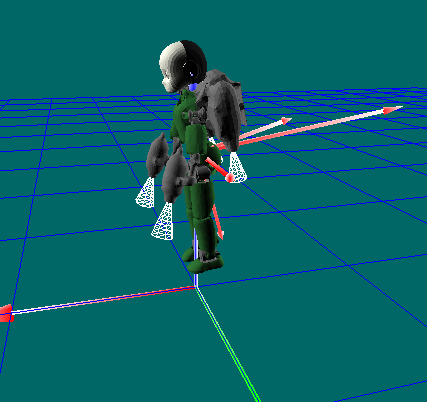
\includegraphics[width=30mm]{./imagines/arrow.png}}
        \subfigure[]{\label{}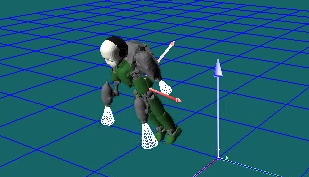
\includegraphics[width=50mm]{./imagines/pitch_down.png}}
    \caption{a) Scenario 1; b) Scenario 2, with the aerodynamic force vector and body frame shown as arrows on the body.} 
    \label{fig:scen}
\end{figure}

%\begin{figure}[t]
%      \centering
%      
\includegraphics[width=60mm]{./imagines/vcom.eps}
%     \caption{robot's CoM velocity profile w.r.t. the inertial frame}
%     \label{fig:motion}
%\end{figure}

\subsection{Robustness Analysis with No Aerodynamics Awareness}

\begin{figure}[t]
    \centering
        \subfigure[]{\label{fig:h_rob}
\includegraphics[width=40mm]{./imagines/pos_linMom_noaf_af.eps}}
        \subfigure[]{\label{fig:hf_rob}
\includegraphics[width=40mm]{./imagines/pos_linMom_noaf_af_hs.eps}}
    \caption{a) Hovering scenario: flight controller that does not account for aerodynamics, with (red line) and without (blue line) aerodynamic effects acting on the system; b) High-speed scenario: flight controller that does not account for aerodynamics, with (red line) and without (blue line) aerodynamic effects acting on the system.} 
    \label{fig:af_no}
\end{figure}



% \begin{figure}[t]
%       \centering
%       
\includegraphics[width=60mm]{./imagines/pos_linMom_noaf_af.eps}
%       \caption{Hovering scenario: flight controller that does not account for aerodynamics, with (red line) and without (blue line) aerodynamic effects acting on the system.} 
%       \label{fig:h_rob} 
% \end{figure}

% \begin{figure}[t]
%       \centering
%       
\includegraphics[width=60mm]{./imagines/pos_linMom_noaf_af_hs.eps}
%       \caption{High-speed scenario: flight controller that does not account for aerodynamics, with (red line) and without (blue line) aerodynamic effects acting on the system.} 
%       \label{fig:hf_rob} 
% \end{figure}

We first evaluate the performances of the baseline controller presented in \cite{c1}\cite{c2} for the designed flight envelope. The controller has been fine tuned to achieve the best performances possible without aerodynamics effects. 

Simulation results are presented in Fig.~\ref{fig:af_no}. We focus our attention on the CoM and linear momentum error norm, which are significantly affected by the disturbance introduced by the wind. As depicted by Fig. \ref{fig:h_rob}, the robot is still able to hover despite the presence of the wind. However, the CoM error norm considerably increases, with a peak of $\SI{30}{cm}$ error and a constant error of about $\SI{3}{cm}$. For what concerns instead the high-speed flight scenario, for which robot control is more critical because the system dynamics are more excited, the controller is not able to retain stability in presence of wind, and the robot crashes on ground, as shown by Fig.~\ref{fig:hf_rob}. 

%At first, we performed simulations for hovering and high-speed flight conditions without considering aerodynamic forces which are the reference conditions for the analysis of aerodynamic effects on the robot, see Fig. \ref{fig:a1}, \ref{fig:c1}, \ref{fig:a2} and \ref{fig:c2}. We proceeded the robustness analysis for hovering and high-speed flight cases individually by testing the wind gust range (starting from the constant wind speed $\SI{3}{m/s}$ to the maximum wind gust value) inside which the robot can stabilize. With the wind velocity along the $-\boldsymbol{X}$ axis of the inertial frame $\mathcal{I}$, the maximum wind gust value is $\SI{53}{m/s}$ for hovering case and $\SI{9}{m/s}$ for high-speed flight. The results in Fig. \ref{fig:b1}, \ref{fig:d1}, \ref{fig:b2} and \ref{fig:d2} represent the CoM position error norm and linear momentum error norm with the air environment described in Fig. \ref{fig:wind}. The results show that with a maximum wind gust value as $\SI{10}{m/s}$, the CoM position error norm in hovering case increases evidently under the wind gust impact but it converges to equilibrium point after the wind impact; in high-speed flight case, the control outputs diverge and the robot loses stability. The limitations of current controller while handling aerodynamic effects caused by wind gust impact are pointed out.

% \begin{figure}[t]
%     \centering
%         \subfigure[]{\label{fig:a1}
\includegraphics[width=40mm]{./imagines/pos_err_norm_h.eps}}
%         \subfigure[]{\label{fig:b1}
\includegraphics[width=40mm]{./imagines/pos_err_norm_0h.eps}}
%         \subfigure[]{\label{fig:c1}
\includegraphics[width=40mm]{./imagines/linMom_err_norm_h.eps}}
%         \subfigure[]{\label{fig:d1}
\includegraphics[width=40mm]{./imagines/linMom_err_norm_0h.eps}}
%     \caption{Hovering: a) and c) without aerodynamic effects; b) and d) with aerodynamic effects}
%     \label{fig:h_rob}
%\end{figure}
% \begin{figure}[t]
%     \centering
%         \subfigure[]{\label{fig:a2}
\includegraphics[width=40mm]{./imagines/pos_err_norm_f.eps}}
%         \subfigure[]{\label{fig:b2}
\includegraphics[width=40mm]{./imagines/pos_err_norm_0f.eps}}
%         \subfigure[]{\label{fig:c2}
\includegraphics[width=40mm]{./imagines/linMom_err_norm_f.eps}}
%         \subfigure[]{\label{fig:d2}
\includegraphics[width=40mm]{./imagines/linMom_err_norm_0f.eps}}
%     \caption{High-speed flight: a) and c) without aerodynamic effects; b) and d) with aerodynamic effects} 
%     \label{fig:hf_rob}
% \end{figure}

\subsection{Control Results with Aerodynamics Awareness}
\label{subsec:ctrl-results-aerodyn}
The two scenarios in the flight envelope are then tested with the flight controller modifications proposed in Sec. \ref{sec:control}. Results are presented in Fig.~\ref{fig:fl_gs}, that show the CoM and linear momentum error norm during the flight simulations. In the hovering scenario depicted in Fig.~\ref{fig:h_control}, the feedback linearization controller (red line) manages to considerably reduce the CoM error despite the external disturbances. However, the closed-loop system dynamics presents oscillations, visible in particular in the linear momentum error plot in Fig.~\ref{fig:h_control}. To fairly compare the results of feedback linearization controller with the baseline controller previously developed, we did not perform any change in the controller's gains: we believe that this oscillation could be mitigated by re-tuning all the gains for this new controller. On the other side, gain scheduling helped to reduce the maximum CoM position error by $\sim 38 \%$ w.r.t. the baseline controller during the wind gust. 

In the high-speed scenario of Fig. \ref{fig:hf_control}, both controllers are able to retain system stability despite the presence of wind. Feedback linearization control also allows to maintain small CoM and linear momentum error norm during the whole simulation. In gain scheduling case, we decided to reduce the CoM gains while the wind gust occurs. The gains relaxation allows to preserve robot control at the cost of a large errors on the CoM position. Fig. \ref{fig:raise gain} shows how the elements of the gains matrix $K_I$ vary for both reference scenarios.\looseness=-1

The performances of the baseline and aerodynamics-aware controllers are briefly compared and summarized in Table \ref{table:comp}, and a video describing the performed simulations is attached to the paper.

%To compare the performances of the robot with different control techniques, the air environment in the simulations is the same as in Fig. \ref{fig:wind}. The results are in Fig. \ref{fig:h_control} and \ref{fig:hf_control}, that presents the CoM position $\&$ linear momentum error norm for both hovering and high-speed flight cases implemented with gain-scheduling and feedback linearization individually. The reduction of CoM position error norm in hovering case varies quite much between the two control techniques applied; the maximum wind gust value under which the robot can stabilize during high-speed flight is increased to $\SI{10}{m/s}$ by applying gain-scheduling and to $\SI{13}{m/s}$ by applying feedback linearization. The percentage that describes the improvements of the controller is presented in Table \ref{table:comp} and the feedback control technique returns better performance in sense of overcoming the limitations of current controller considering aerodynamic effects.

\begin{table}[t]
\vspace*{0.3cm}
\caption{Gain-scheduling V.S. Feedback linearization}
\label{table:comp}
\begin{center}
\begin{tabular}{c|c|c}
\toprule
\multirow{2}{*} & Max-pos-err: & Max-wind-gust: \\ 
 & hovering & high-speed flight \\
\midrule
Current controller & $\SI{0.29}{m}$ & $\SI{9}{m/s}$\\
\midrule
 Gain-scheduling  & $\SI{0.18}{m}$ ($-38\%$) & $\SI{10}{m/s}$ ($+11\%$)\\
\midrule
Feedback linearization & $\SI{0.035}{m}$ ($-88\%$) & $\SI{13}{m/s}$ ($+44\%$)\\
\bottomrule
\end{tabular}
\end{center}
\end{table}

\begin{figure}[t]
    \centering
        \subfigure[]{\label{fig:h_control}
\includegraphics[width=40mm]{./imagines/pos_linMom_fl_2h.eps}}
        \subfigure[]{\label{fig:hf_control}
\includegraphics[width=40mm]{./imagines/pos_linMom_fl_1f.eps}}
    \caption{a) Hovering Scenario: gain-scheduling (blue) V.S. feedback linearization (red); b) High-speed scenario: gain-scheduling (blue) V.S. feedback linearization (red).} 
    \label{fig:fl_gs}
\end{figure}




% \begin{figure}[t]
%       \centering
%       
\includegraphics[width=60mm]{./imagines/pos_linMom_fl_2h.eps}
%       \caption{Hovering Scenario: gain-scheduling (blue) V.S. feedback linearization (red)} 
%       \label{fig:h_control} 
% \end{figure}

% \begin{figure}[t]
%       \centering
%       
\includegraphics[width=60mm]{./imagines/pos_linMom_fl_1f.eps}
%       \caption{High-speed scenario: gain-scheduling (blue) V.S. feedback linearization (red)} 
%       \label{fig:hf_control} 
% \end{figure}

% \begin{figure}[t]
%     \centering
%         \subfigure[]{\label{fig:a3}
\includegraphics[width=40mm]{./imagines/pos_err_norm_2h.eps}}
%         \subfigure[]{\label{fig:b3}
\includegraphics[width=40mm]{./imagines/pos_err_norm_fl_0h.eps}}
%         \subfigure[]{\label{fig:c3}
\includegraphics[width=40mm]{./imagines/linMom_err_norm_2h.eps}}
%         \subfigure[]{\label{fig:d3}
\includegraphics[width=40mm]{./imagines/linMom_err_norm_fl_0h.eps}}
%     \caption{Hovering: a) and c) gain-scheduling; b) and d) feedback linearization} 
%     \label{fig:h_control}
% \end{figure}

% \begin{figure}[t]
%     \centering
%         \subfigure[]{\label{fig:a4}
\includegraphics[width=40mm]{./imagines/pos_err_norm_1f.eps}}
%         \subfigure[]{\label{fig:b4}
\includegraphics[width=40mm]{./imagines/pos_err_norm_fl_0f.eps}}
%         \subfigure[]{\label{fig:c4}
\includegraphics[width=40mm]{./imagines/linMom_err_norm_1f.eps}}
%         \subfigure[]{\label{fig:d4}
\includegraphics[width=40mm]{./imagines/linMom_err_norm_fl_0f.eps}}
%     \caption{High-speed flight: a) and c) gain-scheduling; b) and d) feedback linearization} 
%     \label{fig:hf_control}
% \end{figure}
